% Options for packages loaded elsewhere
% Options for packages loaded elsewhere
\PassOptionsToPackage{unicode}{hyperref}
\PassOptionsToPackage{hyphens}{url}
%
\documentclass[
  ignorenonframetext,
]{beamer}
\newif\ifbibliography
\usepackage{pgfpages}
\setbeamertemplate{caption}[numbered]
\setbeamertemplate{caption label separator}{: }
\setbeamercolor{caption name}{fg=normal text.fg}
\beamertemplatenavigationsymbolsempty
% remove section numbering
\setbeamertemplate{part page}{
  \centering
  \begin{beamercolorbox}[sep=16pt,center]{part title}
    \usebeamerfont{part title}\insertpart\par
  \end{beamercolorbox}
}
\setbeamertemplate{section page}{
  \centering
  \begin{beamercolorbox}[sep=12pt,center]{section title}
    \usebeamerfont{section title}\insertsection\par
  \end{beamercolorbox}
}
\setbeamertemplate{subsection page}{
  \centering
  \begin{beamercolorbox}[sep=8pt,center]{subsection title}
    \usebeamerfont{subsection title}\insertsubsection\par
  \end{beamercolorbox}
}
% Prevent slide breaks in the middle of a paragraph
\widowpenalties 1 10000
\raggedbottom
\AtBeginPart{
  \frame{\partpage}
}
\AtBeginSection{
  \ifbibliography
  \else
    \frame{\sectionpage}
  \fi
}
\AtBeginSubsection{
  \frame{\subsectionpage}
}
\usepackage{iftex}
\ifPDFTeX
  \usepackage[T1]{fontenc}
  \usepackage[utf8]{inputenc}
  \usepackage{textcomp} % provide euro and other symbols
\else % if luatex or xetex
  \usepackage{unicode-math} % this also loads fontspec
  \defaultfontfeatures{Scale=MatchLowercase}
  \defaultfontfeatures[\rmfamily]{Ligatures=TeX,Scale=1}
\fi
\usepackage{lmodern}

\usetheme[]{slides\_theme.scss}
\ifPDFTeX\else
  % xetex/luatex font selection
\fi
% Use upquote if available, for straight quotes in verbatim environments
\IfFileExists{upquote.sty}{\usepackage{upquote}}{}
\IfFileExists{microtype.sty}{% use microtype if available
  \usepackage[]{microtype}
  \UseMicrotypeSet[protrusion]{basicmath} % disable protrusion for tt fonts
}{}
\makeatletter
\@ifundefined{KOMAClassName}{% if non-KOMA class
  \IfFileExists{parskip.sty}{%
    \usepackage{parskip}
  }{% else
    \setlength{\parindent}{0pt}
    \setlength{\parskip}{6pt plus 2pt minus 1pt}}
}{% if KOMA class
  \KOMAoptions{parskip=half}}
\makeatother


\usepackage{longtable,booktabs,array}
\usepackage{calc} % for calculating minipage widths
\usepackage{caption}
% Make caption package work with longtable
\makeatletter
\def\fnum@table{\tablename~\thetable}
\makeatother
\usepackage{graphicx}
\makeatletter
\newsavebox\pandoc@box
\newcommand*\pandocbounded[1]{% scales image to fit in text height/width
  \sbox\pandoc@box{#1}%
  \Gscale@div\@tempa{\textheight}{\dimexpr\ht\pandoc@box+\dp\pandoc@box\relax}%
  \Gscale@div\@tempb{\linewidth}{\wd\pandoc@box}%
  \ifdim\@tempb\p@<\@tempa\p@\let\@tempa\@tempb\fi% select the smaller of both
  \ifdim\@tempa\p@<\p@\scalebox{\@tempa}{\usebox\pandoc@box}%
  \else\usebox{\pandoc@box}%
  \fi%
}
% Set default figure placement to htbp
\def\fps@figure{htbp}
\makeatother


% definitions for citeproc citations
\NewDocumentCommand\citeproctext{}{}
\NewDocumentCommand\citeproc{mm}{%
  \begingroup\def\citeproctext{#2}\cite{#1}\endgroup}
\makeatletter
 % allow citations to break across lines
 \let\@cite@ofmt\@firstofone
 % avoid brackets around text for \cite:
 \def\@biblabel#1{}
 \def\@cite#1#2{{#1\if@tempswa , #2\fi}}
\makeatother
\newlength{\cslhangindent}
\setlength{\cslhangindent}{1.5em}
\newlength{\csllabelwidth}
\setlength{\csllabelwidth}{3em}
\newenvironment{CSLReferences}[2] % #1 hanging-indent, #2 entry-spacing
 {\begin{list}{}{%
  \setlength{\itemindent}{0pt}
  \setlength{\leftmargin}{0pt}
  \setlength{\parsep}{0pt}
  % turn on hanging indent if param 1 is 1
  \ifodd #1
   \setlength{\leftmargin}{\cslhangindent}
   \setlength{\itemindent}{-1\cslhangindent}
  \fi
  % set entry spacing
  \setlength{\itemsep}{#2\baselineskip}}}
 {\end{list}}
\usepackage{calc}
\newcommand{\CSLBlock}[1]{\hfill\break\parbox[t]{\linewidth}{\strut\ignorespaces#1\strut}}
\newcommand{\CSLLeftMargin}[1]{\parbox[t]{\csllabelwidth}{\strut#1\strut}}
\newcommand{\CSLRightInline}[1]{\parbox[t]{\linewidth - \csllabelwidth}{\strut#1\strut}}
\newcommand{\CSLIndent}[1]{\hspace{\cslhangindent}#1}



\setlength{\emergencystretch}{3em} % prevent overfull lines

\providecommand{\tightlist}{%
  \setlength{\itemsep}{0pt}\setlength{\parskip}{0pt}}



 


\makeatletter
\@ifpackageloaded{caption}{}{\usepackage{caption}}
\AtBeginDocument{%
\ifdefined\contentsname
  \renewcommand*\contentsname{Table of contents}
\else
  \newcommand\contentsname{Table of contents}
\fi
\ifdefined\listfigurename
  \renewcommand*\listfigurename{List of Figures}
\else
  \newcommand\listfigurename{List of Figures}
\fi
\ifdefined\listtablename
  \renewcommand*\listtablename{List of Tables}
\else
  \newcommand\listtablename{List of Tables}
\fi
\ifdefined\figurename
  \renewcommand*\figurename{Figure}
\else
  \newcommand\figurename{Figure}
\fi
\ifdefined\tablename
  \renewcommand*\tablename{Table}
\else
  \newcommand\tablename{Table}
\fi
}
\@ifpackageloaded{float}{}{\usepackage{float}}
\floatstyle{ruled}
\@ifundefined{c@chapter}{\newfloat{codelisting}{h}{lop}}{\newfloat{codelisting}{h}{lop}[chapter]}
\floatname{codelisting}{Listing}
\newcommand*\listoflistings{\listof{codelisting}{List of Listings}}
\makeatother
\makeatletter
\makeatother
\makeatletter
\@ifpackageloaded{caption}{}{\usepackage{caption}}
\@ifpackageloaded{subcaption}{}{\usepackage{subcaption}}
\makeatother
\makeatletter
\@ifpackageloaded{sidenotes}{}{\usepackage{sidenotes}}
\@ifpackageloaded{marginnote}{}{\usepackage{marginnote}}
\makeatother

\usepackage{bookmark}
\IfFileExists{xurl.sty}{\usepackage{xurl}}{} % add URL line breaks if available
\urlstyle{same}
\hypersetup{
  pdftitle={Sprachverarbeitung und Spracherwerb aus typologischer Sicht},
  pdfauthor={Eva Scheel},
  hidelinks,
  pdfcreator={LaTeX via pandoc}}


\title{Sprachverarbeitung und Spracherwerb aus typologischer Sicht}
\subtitle{Sitzung 1: Einführung}
\author{Eva Scheel}
\date{}
\institute{eva.scheel-huber@uni-koeln.de}

\begin{document}
\frame{\titlepage}


\begin{frame}
\begin{block}{Übersicht}
\phantomsection\label{uxfcbersicht}
\begin{itemize}
\tightlist
\item
  Vorstellungsrunde
\item
  Informationen zum Kurs
\item
  Übersicht und Leistungsnachweise
\item
  Einführung ins Thema
\end{itemize}
\end{block}

\begin{block}{Ziele von heute sind, dass \ldots{}}
\phantomsection\label{ziele-von-heute-sind-dass}
\begin{itemize}[<+->]
\tightlist
\item
  wir uns kennenlernen
\item
  Sie einen Überblick über den Verlauf des Kurses und die Anforderungen
  haben
\item
  wissen, was wir in der Psycholinguistik erforschen und \ldots{}
\item
  \ldots{} mit was wir uns hier spezifisch im Seminar befassen werden
\end{itemize}
\end{block}

\begin{block}{Vorstellungsrunde}
\phantomsection\label{vorstellungsrunde}
\begin{itemize}
\tightlist
\item
  Name \& wie Sie angesprochen werden wollen
\item
  Studiengang
\item
  Grund für die Wahl des Kurses
\item
  Sprachen, die Sie sprechen, oder die Sie gerne lernen würden
\end{itemize}
\end{block}

\begin{block}{Allgemeine Informationen}
\phantomsection\label{allgemeine-informationen}
\begin{itemize}
\tightlist
\item
  Donnerstag, 14:00-15:30, Seminarraum rechts
\item
  Keine Sprechstunde, kontaktieren Sie mich per Email
\item
  Folien und Seminar auf Deutsch, Lektüre vorwiegend auf Englisch
\item
  Seminar im SM1:

  \begin{itemize}
  \tightlist
  \item
    Kontaktzeit: 30h
  \item
    Selbststudium: 60h
  \end{itemize}
\end{itemize}
\end{block}
\end{frame}

\begin{frame}
\begin{block}{Form des Seminars}
\phantomsection\label{form-des-seminars}
\begin{itemize}
\tightlist
\item
  hauptsächlich Lesen und Diskutieren von Artikeln aus Fachzeitschriften
\item
  d.h. wenig Frontalunterricht
\end{itemize}
\end{block}

\begin{block}{Frage an Sie}
\phantomsection\label{frage-an-sie}
\textbf{Was wünschen Sie sich für eine angenehme und produktive
Zusammenarbeit?}

\href{link}{Link}
\end{block}

\begin{block}{Was ich von Ihnen erwarte}
\phantomsection\label{was-ich-von-ihnen-erwarte}
\begin{itemize}[<+->]
\tightlist
\item
  respektvollen Umgang, es ist mir wichtig das alle sich wohl fühlen
\item
  Unterschiede und Diversität wird als Gewinn und nicht als Nachteil
  betracht
\item
  nutzen Sie die Gelegenheit im Unterricht Fragen zu stellen, Meinungen
  zu äußern, zu diskutieren und so zu lernen. Es gibt keine ``doofen''
  Fragen \& Kommentare.
\item
  Diversität?
\item
  Rückmeldungen, Ideen und Anregungen Ihrerseits sind erwünscht!
\item
  Dieses Seminar ist abhängig von Ihrer Anwesenheit und aktiven
  Mitarbeit. Ihre Anwesenheit in den Sitzungen wird deshalb erwartet.

  \begin{itemize}[<+->]
  \tightlist
  \item
    bei Abwesenheit, melden Sie sich bitte vorab bei mir
  \end{itemize}
\item
  Falls Sie eine Sitzung verpassen, informieren Sie sich bei Ihren
  Kommiliton:innen, nicht alle Informationen können auf den Folien
  gefunden werden
\item
  um die ``aktive Teilnahme'' zu erhalten: Erbringung der
  Leistungsnachweise
\item
  Prüfungsleistung: Hausarbeit
\end{itemize}
\end{block}

\begin{block}{Wochenplan}
\phantomsection\label{wochenplan}
\end{block}

\begin{block}{Leistungsnachweise*}
\phantomsection\label{leistungsnachweise}
\begin{columns}[T]
\begin{column}{0.5\linewidth}
{\textbf{Leistungsnachweis A}}

\begin{itemize}[<+->]
\tightlist
\item
  Artikel lesen und Fragen/Diskussionspunkte vor der Sitzung online
  teilen, auf andere Kommentare Bezug nehmen und andere Fragen
  beantworten
\item
  für den Leistungsnachweis: 5/6 Beiträge sind obligatorisch
\end{itemize}
\end{column}

\begin{column}{0.5\linewidth}
{\textbf{Leistungsnachweis B}}

\begin{itemize}[<+->]
\tightlist
\item
  kleine Projektarbeit in Gruppen oder alleine
\item
  Vorstellen am Ende des Semesters
\item
  Inhalt: Übertragen einer Studie in eine andere Sprache
\end{itemize}
\end{column}
\end{columns}

\marginnote{\begin{footnotesize}

*für die aktive Teilnahme

\end{footnotesize}}
\end{block}

\begin{block}{Einführung}
\phantomsection\label{einfuxfchrung}
\textbf{Mit was beschäftigen wir uns in der Psycholinguistik?}

\begin{itemize}
\tightlist
\item
  kognitive Vorgänge und Zustände des sprachlichen Wissens
\item
  Spracherwerb
\item
  Sprachproduktion
\item
  Sprachverstehen
\item
  Sprachstörungen
\end{itemize}

Dietrich and Gerwien (2017)
\end{block}
\end{frame}

\begin{frame}
\begin{block}{Kognitive Vorgänge (``Mechanismen'') und Zustände des
sprachlichen Wissens}
\phantomsection\label{kognitive-vorguxe4nge-mechanismen-und-zustuxe4nde-des-sprachlichen-wissens}
Was sind die Komponenten des sprachlichen Wissens?

\begin{itemize}[<+->]
\tightlist
\item
  lexikalische Wissen
\item
  grammatischen Kombinatorik (oder einfach nur ``Grammatik'')
\end{itemize}

Was sind mögliche Prozeduren, Mechanismen?

\begin{itemize}[<+->]
\tightlist
\item
  Sprache verstehen
\item
  Sprache produzieren
\item
  nicht identische Mechanismen!
\end{itemize}

Dietrich and Gerwien (2017)

\note{kognitive Vorgänge und Zustände des sprachlichen Wissens:
Sprachfähigkeit des Menschen beruht auf dem Zusammenwirken mehrerer
Wissensbestände und Verarbeitungssysteme

lexikalische Wissen: Bedeutung, syntaktische Eigenschaften, Morphologie
(``innerer Aufbau''), Ausdrucksseite

grammatische Kombinatorik: prozedurales Wissen um das Zusammenpassen
sprachlicher Einheiten unter strukturellen Bedingungen}
\end{block}
\end{frame}

\begin{frame}
{\textbf{Sprachfähigkeit}: Wechselwirkung zwischen Sprachwissen und
Sprachvorgängen}

Dietrich and Gerwien (2017)
\end{frame}

\begin{frame}
\begin{block}{Spracherwerb}
\phantomsection\label{spracherwerb}
\textbf{Wie wird das sprachliche Wissen und die Sprachvorgänge erworben?
Wie entwickeln sie sich?}

{Beispiele?}

\begin{itemize}[<+->]
\tightlist
\item
  Wie werden Wörter gelernt?

  \begin{itemize}[<+->]
  \tightlist
  \item
    Wie werden die Regeln gelernt wie Wörter geformt werden? kombiniert
    werden?
  \end{itemize}
\item
  Wie werden (komplexe) Satzstrukturen gelernt?
\item
  Wie versteht ein Kind Sätze? Wie lernt es Sätze zu verarbeiten?
\end{itemize}
\end{block}
\end{frame}

\begin{frame}
\begin{block}{Sprachproduktion}
\phantomsection\label{sprachproduktion}
{\textbf{Was sind die kognitive Prozesse die der Sprachproduktion
unterliegen?}}

\begin{figure}[H]

{\centering 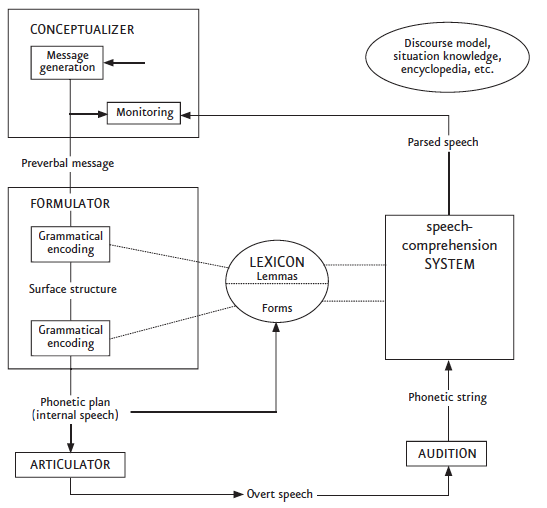
\includegraphics[width=6.875in,height=\textheight,keepaspectratio]{images/leveltsproduction.png}

}

\caption{Levelt's model of speech production Levelt (1989), adaptiert
von Ruiter (1998)}

\end{figure}%

\note{\begin{itemize}
\tightlist
\item
  Conceptualizer: Intention und Message werden geformt

  \begin{itemize}
  \tightlist
  \item
    kommunikatives Ziel (macro)
  \item
    wie Information strukturiert wird (micro)
  \item
    output: ``preverbal message''
  \end{itemize}
\item
  Formulator: Message wird zu einem linguistischen ``Plan'' übersetzt
  (grammatische und phonetische Form)

  \begin{itemize}
  \tightlist
  \item
    grammatical encoding: Wörter finden

    \begin{itemize}
    \tightlist
    \item
      Lemmatas und Formen
    \item
      Syntaktische Struktur
    \end{itemize}
  \item
    phonetische Form wird abgerufen, übergeben an den Articulator
  \end{itemize}
\item
  Articulator: der ``Plan'' wird physisch artikuliert

  \begin{itemize}
  \tightlist
  \item
    Neuronale Signale zu Muskeln (Lunge, Zunge, Kehlkopf)
  \item
  \end{itemize}
\item
  Monitoring:

  \begin{itemize}
  \tightlist
  \item
    wir überprüfen unsere Äußerungen stets
  \item
    intern und extern
  \end{itemize}
\end{itemize}}
\end{block}
\end{frame}

\begin{frame}
\begin{block}{Sprachproduktion}
\phantomsection\label{sprachproduktion-1}
{\textbf{Was sind die kognitive Prozesse die der Sprachproduktion
unterliegen?}}

\begin{figure}[H]

{\centering 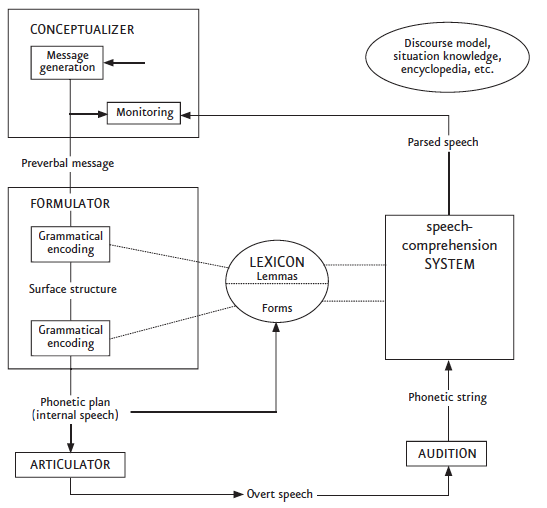
\includegraphics[width=6.875in,height=\textheight,keepaspectratio]{images/leveltsproduction.png}

}

\caption{Levelt's model of speech production Levelt (1989), adaptiert
von Ruiter (1998)}

\end{figure}%

{Was fehlt hier?}
\end{block}
\end{frame}

\begin{frame}
\begin{block}{Sprachverstehen}
\phantomsection\label{sprachverstehen}
{\textbf{Wie funktioniert das Sprachverstehen?}}

\begin{figure}[H]

{\centering 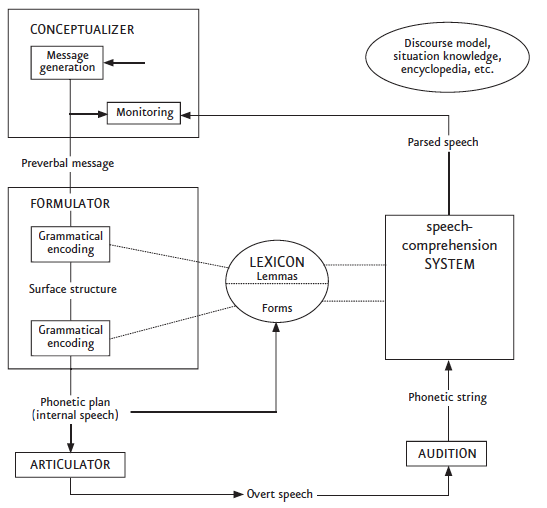
\includegraphics[width=6.875in,height=\textheight,keepaspectratio]{images/leveltsproduction.png}

}

\caption{Levelt (1989), adaptiert von Ruiter (1998)}

\end{figure}%

\note{\begin{itemize}
\tightlist
\item
  Lauterkennung, entnehmen der Lautform des akustischen Ereignisses
\item
  segmentiert werden
\item
  kategoriale Wahrnehmung
\item
  Worterkennung
\item
  die Wörter müssen geparst werden, der syntaktische Aufbau, Verstehen
  wie Wört zusammenhängen
\item
  prosodisches Wissen
\item
  pragmatisches Wissen
\item
  Weltwissen
\end{itemize}}
\end{block}
\end{frame}

\begin{frame}
\begin{block}{Sprachverstehen}
\phantomsection\label{sprachverstehen-1}
{\textbf{Inkrementalität}}
\end{block}
\end{frame}

\begin{frame}
\begin{block}{Sprachstörungen}
\phantomsection\label{sprachstuxf6rungen}
\end{block}

\begin{block}{Einführung}
\phantomsection\label{einfuxfchrung-1}
\textbf{Mit was beschäftigen wir uns in der Psycholinguistik?}

\begin{itemize}
\item
  kognitive Vorgänge und Zustände des sprachlichen Wissens
\item
  {\textbf{Spracherwerb}}
\item
  Sprachproduktion
\item
  {\textbf{Sprachverstehen}}
\item
  Sprachstörungen
\end{itemize}

Dietrich and Gerwien (2017)
\end{block}
\end{frame}

\begin{frame}{Lektürenempfehlungen}
\phantomsection\label{lektuxfcrenempfehlungen}
\end{frame}

\begin{frame}{References}
\phantomsection\label{references}
\phantomsection\label{refs}
\begin{CSLReferences}{1}{0}
\bibitem[\citeproctext]{ref-dietrich2017}
Dietrich, Rainer, and Johannes Gerwien. 2017. \emph{Psycholinguistik}.
Stuttgart: J.B. Metzler.
\url{https://doi.org/10.1007/978-3-476-05494-4}.

\bibitem[\citeproctext]{ref-levelt1989}
Levelt, Willem J. M. 1989. \emph{Speaking: From Intention to
Articulation}. The MIT Press.
\url{https://doi.org/10.7551/mitpress/6393.001.0001}.

\bibitem[\citeproctext]{ref-ruiter1998gesture}
Ruiter, Jan Peter de. 1998. \emph{Gesture and Speech Production}.
unpublished dissertation, Nijmegen.

\end{CSLReferences}
\end{frame}




\end{document}
